%File: anonymous-submission-latex-2024.tex
\documentclass[letterpaper]{article} % DO NOT CHANGE THIS
\usepackage[submission]{aaai24}  % DO NOT CHANGE THIS
\usepackage{times}  % DO NOT CHANGE THIS
\usepackage{helvet}  % DO NOT CHANGE THIS
\usepackage{courier}  % DO NOT CHANGE THIS
\usepackage[hyphens]{url}  % DO NOT CHANGE THIS
\usepackage{graphicx} % DO NOT CHANGE THIS
\urlstyle{rm} % DO NOT CHANGE THIS
\def\UrlFont{\rm}  % DO NOT CHANGE THIS
\usepackage{natbib}  % DO NOT CHANGE THIS AND DO NOT ADD ANY OPTIONS TO IT
\usepackage{caption} % DO NOT CHANGE THIS AND DO NOT ADD ANY OPTIONS TO IT
\frenchspacing  % DO NOT CHANGE THIS
\setlength{\pdfpagewidth}{8.5in} % DO NOT CHANGE THIS
\setlength{\pdfpageheight}{11in} % DO NOT CHANGE THIS
%
% These are recommended to typeset algorithms but not required. See the subsubsection on algorithms. Remove them if you don't have algorithms in your paper.
\usepackage{algorithm}
\usepackage{algorithmic}


\usepackage{booktabs}
\usepackage{amsmath}
\usepackage[table]{xcolor}
\usepackage{amssymb}

% added by ns
\usepackage{multirow}
\usepackage{threeparttable}

%
% These are are recommended to typeset listings but not required. See the subsubsection on listing. Remove this block if you don't have listings in your paper.
\usepackage{newfloat}
\usepackage{listings}
\DeclareCaptionStyle{ruled}{labelfont=normalfont,labelsep=colon,strut=off} % DO NOT CHANGE THIS
\lstset{%
	basicstyle={\footnotesize\ttfamily},% footnotesize acceptable for monospace
	numbers=left,numberstyle=\footnotesize,xleftmargin=2em,% show line numbers, remove this entire line if you don't want the numbers.
	aboveskip=0pt,belowskip=0pt,%
	showstringspaces=false,tabsize=2,breaklines=true}
\floatstyle{ruled}
\newfloat{listing}{tb}{lst}{}
\floatname{listing}{Listing}
%
% Keep the \pdfinfo as shown here. There's no need
% for you to add the /Title and /Author tags.
\pdfinfo{
/TemplateVersion (2024.1)
}

% DISALLOWED PACKAGES
% \usepackage{authblk} -- This package is specifically forbidden
% \usepackage{balance} -- This package is specifically forbidden
% \usepackage{color (if used in text)
% \usepackage{CJK} -- This package is specifically forbidden
% \usepackage{float} -- This package is specifically forbidden
% \usepackage{flushend} -- This package is specifically forbidden
% \usepackage{fontenc} -- This package is specifically forbidden
% \usepackage{fullpage} -- This package is specifically forbidden
% \usepackage{geometry} -- This package is specifically forbidden
% \usepackage{grffile} -- This package is specifically forbidden
% \usepackage{hyperref} -- This package is specifically forbidden
% \usepackage{navigator} -- This package is specifically forbidden
% (or any other package that embeds links such as navigator or hyperref)
% \indentfirst} -- This package is specifically forbidden
% \layout} -- This package is specifically forbidden
% \multicol} -- This package is specifically forbidden
% \nameref} -- This package is specifically forbidden
% \usepackage{savetrees} -- This package is specifically forbidden
% \usepackage{setspace} -- This package is specifically forbidden
% \usepackage{stfloats} -- This package is specifically forbidden
% \usepackage{tabu} -- This package is specifically forbidden
% \usepackage{titlesec} -- This package is specifically forbidden
% \usepackage{tocbibind} -- This package is specifically forbidden
% \usepackage{ulem} -- This package is specifically forbidden
% \usepackage{wrapfig} -- This package is specifically forbidden
% DISALLOWED COMMANDS
% \nocopyright -- Your paper will not be published if you use this command
% \addtolength -- This command may not be used
% \balance -- This command may not be used
% \baselinestretch -- Your paper will not be published if you use this command
% \clearpage -- No page breaks of any kind may be used for the final version of your paper
% \columnsep -- This command may not be used
% \newpage -- No page breaks of any kind may be used for the final version of your paper
% \pagebreak -- No page breaks of any kind may be used for the final version of your paperr
% \pagestyle -- This command may not be used
% \tiny -- This is not an acceptable font size.
% \vspace{- -- No negative value may be used in proximity of a caption, figure, table, section, subsection, subsubsection, or reference
% \vskip{- -- No negative value may be used to alter spacing above or below a caption, figure, table, section, subsection, subsubsection, or reference

\setcounter{secnumdepth}{2} %May be changed to 1 or 2 if section numbers are desired.

% The file aaai24.sty is the style file for AAAI Press
% proceedings, working notes, and technical reports.
%

% Title

% Your title must be in mixed case, not sentence case.
% That means all verbs (including short verbs like be, is, using,and go),
% nouns, adverbs, adjectives should be capitalized, including both words in hyphenated terms, while
% articles, conjunctions, and prepositions are lower case unless they
% directly follow a colon or long dash
%\title{Mining Fine-Grained Image-Text Alignment in CLIP for Zero-Shot Captioning via Text-Only Training}
\title{Mining Fine-Grained Image-Text Alignment for Zero-Shot Captioning via Text-Only Training}
\author{
    %Authors
    % All authors must be in the same font size and format.
    Written by AAAI Press Staff\textsuperscript{\rm 1}\thanks{With help from the AAAI Publications Committee.}\\
    AAAI Style Contributions by Pater Patel Schneider,
    Sunil Issar,\\
    J. Scott Penberthy,
    George Ferguson,
    Hans Guesgen,
    Francisco Cruz\equalcontrib,
    Marc Pujol-Gonzalez\equalcontrib
}
\affiliations{
    %Afiliations
    \textsuperscript{\rm 1}Association for the Advancement of Artificial Intelligence\\
    % If you have multiple authors and multiple affiliations
    % use superscripts in text and roman font to identify them.
    % For example,

    % Sunil Issar\textsuperscript{\rm 2},
    % J. Scott Penberthy\textsuperscript{\rm 3},
    % George Ferguson\textsuperscript{\rm 4},
    % Hans Guesgen\textsuperscript{\rm 5}
    % Note that the comma should be placed after the superscript

    1900 Embarcadero Road, Suite 101\\
    Palo Alto, California 94303-3310 USA\\
    % email address must be in roman text type, not monospace or sans serif
    proceedings-questions@aaai.org
%
% See more examples next
}

%Example, Single Author, ->> remove \iffalse,\fi and place them surrounding AAAI title to use it
\iffalse
\title{My Publication Title --- Single Author}
\author {
    Author Name
}
\affiliations{
    Affiliation\\
    Affiliation Line 2\\
    name@example.com
}
\fi

\iffalse
%Example, Multiple Authors, ->> remove \iffalse,\fi and place them surrounding AAAI title to use it
\title{My Publication Title --- Multiple Authors}
\author {
    % Authors
    First Author Name\textsuperscript{\rm 1},
    Second Author Name\textsuperscript{\rm 2},
    Third Author Name\textsuperscript{\rm 1}
}
\affiliations {
    % Affiliations
    \textsuperscript{\rm 1}Affiliation 1\\
    \textsuperscript{\rm 2}Affiliation 2\\
    firstAuthor@affiliation1.com, secondAuthor@affilation2.com, thirdAuthor@affiliation1.com
}
\fi


% REMOVE THIS: bibentry
% This is only needed to show inline citations in the guidelines document. You should not need it and can safely delete it.
\usepackage{bibentry}
% END REMOVE bibentry

\begin{document}

\maketitle

\begin{abstract}
%Prior works in image conditioned text generation rely on end-to-end training with annotated caption data, which is expensive and computationally intensive.

% chatgpt refined
% Large-scale pre-trained language models (e.g.,GPT) have shown remarkable conversational and reasoning capabilities across many domains. 
% Recent studies has demonstrated the potential of leveraging CLIP latents to extend the capabilities of large language models to vision language tasks(e.g. image captioning) with text-only training. 
% Despite promising results of previous works, there remains a lack of a comprehensive and unified explanation of the prior approaches used and how CLIP latents can be fully leveraged in these applications.

Image captioning aims at generating descriptive and meaningful textual descriptions of images, enabling a broad range of vision-language applications. Prior works have demonstrated that harnessing the power of Contrastive Image Language Pre-training (CLIP) offers a promising approach to achieving zero-shot captioning, eliminating the need for expensive caption annotations. However, the widely observed modality gap in the latent space of CLIP harms the performance of zero-shot captioning by breaking the alignment between paired image-text features. To address this issue, we conduct an analysis on the CLIP latent space which leads to two findings. Firstly, we observe that the CLIP's visual feature of image subregions can achieve closer proximity to the paired caption due to the inherent information loss in text descriptions. In addition, we show that the modality gap between a paired image-text can be empirically modeled as a zero-mean Gaussian distribution. Motivated by the findings, we propose a novel zero-shot image captioning framework with text-only training to reduce the modality gap. In particular, we introduce a subregion feature aggregation to leverage local region information, which produces a compact visual representation for matching text representation. Moreover, we incorporate a noise injection and CLIP reranking strategy to boost captioning performance. We also extend our framework to build a zero-shot VQA pipeline, demonstrating its generality. Through extensive experiments on common captioning and VQA datasets such as MSCOCO, Flickr30k and VQAV2, we show that our method achieves remarkable performance improvements. Code is available at https://github.com/Artanic30/MacCap.

\end{abstract}
\section{Introduction}
From cleaning robots to self-driving cars, autonomous and semi-autonomous agents are becoming increasingly prevalent~\cite{stone2016artificial}. People's understanding of such agents' behaviors can increase their trust in the agents and their ability to collaborate with them~\cite{devin2016implemented,glass2008toward}. An understanding of an agent's behavior could also support people in tasks such as choosing between alternative agents and determining when the agent can be trusted with performing a task autonomously and when the user's attention is needed. For example, if a user can anticipate the behavior of  a self-driving car in different scenarios, she could be more prepared to take control in situations where the car might not perform well on its own.

While prior work has suggested ways to explain individual decisions of an agent to a person~\cite{khan2009minimal,khan2011automatically}, these approaches do not convey a ``global'' view of an agent's policy. Similarly, recent methods for interpretable machine learning~\cite{vellido2012making,doshi2017towards} typically explain a single decision made by a model, e.g. by presenting a simplified model which justifies decisions in a certain region in the space~\cite{ribeiro2016model}. In this paper, we introduce the problem of providing users with a summary of an agent's behavior. This approach aims to provide users with an overview of the agent's global strategy rather than explaining specific decisions  after the fact. 

A trivial way of communicating an agent's behavior is to show past executions or simulations. This approach, however, has important drawbacks. First, many of the situations an agent encounters might be uninteresting to a person (e.g., a self-driving car stuck in traffic for an hour). Second, reviewing long execution traces will require a person to spend a significant amount of time, and people might give up early, or not pay attention, potentially missing important states. Therefore, we seek solutions that extract \emph{effective} summaries which show the actions taken by the agent in key scenarios. Such summaries can reduce the human effort required to review the agent's behavior, while still providing sufficient information about its capabilities. We note that this is analogous to the approach taken in many settings in which people need to assess the performance of other people. For example, sports scouting agencies typically prepare videos that include highlights from players' games to demonstrate their skills\footnote{e.g.,  \url{https://www.youtube.com/watch?v=gX3e0UM-OeM}. We note that while such scouting videos are often biased to showcase only successful actions, we intend that summaries of agent behavior will include states that demonstrates their behavior in different states of interest, whether successful or not.}.  

%The approach of generating summaries that highlight the capabilities of agents is analogous to other settings in which people need to review the performance of other people. For example, sports scouting agencies prepare videos that include highlights from players' games to demonstrate their skills.\footnote{e.g.,  \url{https://www.youtube.com/watch?v=gX3e0UM-OeM}.}

We developed ``HIGHLIGHTS'', an algorithm that extracts important states from an execution trace of an agent in an online manner. Intuitively, a state is important if different actions in that states can lead to substantially different outcomes for the agent. For example, deciding which turn to take when driving in a city will not be considered important if taking the next turn will result in a similar arrival time; deciding whether to exit a highway will be considered more important, as missing the exit can result in a significant delay. Our approach assumes that HIGHLIGHTS has access to the agent's strategy which is described using a  Markov Decision Process (MDP) policy, and quantifies the importance of states based on the agent's Q-values. To provide more context to the user, rather than showing important states in isolation, the algorithm extracts a trajectory that includes neighboring states and composes a summary of the agent's behavior from these trajectories.

We used HIGHLIGHTS to create summaries of agents playing Mrs. Pacman~\cite{rohlfshagen2011ms} and evaluated these summaries in a human-subject experiment. We compared HIGHLIGHTS summaries with two baselines. One baseline generated summaries by extracting random trajectories of the agent, which will, on average, include states that are more likely to be encountered. The other baseline generated summaries by extracting the first trajectories the agent encountered, which is akin to having a user watch the agent until she runs out of time. In the experiment, participants were shown summaries of different Pacman agents which varied in their performance, and were asked to select an agent to play on their behalf.  They were also asked to rate the helpfulness of different summaries for evaluating an agent's capabilities. 
%They were also shown pairs of summaries of the \emph{same} Pacman agent and were asked to subjectively assess how helpful each of the summaries is for understanding that agent's capabilities. 
Our results show that HIGHLIGHTS led to improved objective performance of participants: they were significantly more likely to choose the better performing agent when the HIGHLIGHTS summaries were shown. HIGHLIGHTS summaries were also rated as more helpful by the study participants. 

%can be condensed to two sentences if needed
One limitation of the HIGHLIGHTS algorithm is that it does not consider the diversity of states in the summary, and therefore if important states are similar to each other, the summary will consist of similar trajectories, thus conveying less new information to users. To mitigate this problem, we developed a variant of the HIGHLIGHTS algorithm which, in addition to state importance, takes into consideration the similarity of the state to other states in the summary. This extension further improved participants' ability to assess the performance of different agents.

The contributions of the paper are threefold: (1) we introduce and formalize the problem of summarizing an agent's behavior to people; (2) we develop HIGHLIGHTS and HIGHLIGHTS-DIV, algorithms that automatically extract summaries of an agent's policy, and (3) we conduct human-subject experiments, showing that summaries generated by HIGHLIGHTS and HIGHLIGHTS-DIV were preferred by participants and improved their ability to assess the capabilities of agents compared to the baseline summaries.

\section{Related Work}
In this section, we briefly review some existing neural matching models and graph neural networks.

\subsection{Neural Matching Models}
Most neural matching models fall within two categories: representation-focused models, e.g. DSSM \cite{huang2013learning}, ARC-I \cite{hu2014convolutional}, CDSSM \cite{shen2014latent}, and interaction-focused models, e.g. MatchPyramid \cite{pang2016text}, DRMM \cite{guo2016deep}, PACRR \cite{hui2017pacrr}, KNRM \cite{xiong2017end}.

The representation-focused models follow the representation learning approach adopted in many natural language processing tasks. Queries and documents are projected into the same semantic space individually. The cosine similarity is then used between their high-level text representations to produce the final relevance score. For example, DSSM \cite{huang2013learning}, one of the earliest neural relevance matching models, employs simple dense neural layers to learn high-level representations for queries and documents. To enhance the projecting function, ARC-I \cite{hu2014convolutional} and CDSSM \cite{shen2014latent} devoted much effort into convolutional layers later on. 

In comparison, interaction-focused methods model the two text sequences jointly, by directly exploiting detailed query-document interaction signals rather than high-level representations of individual texts. For example, DRMM \cite{guo2016deep} maps the local query-document interaction signals into a fixed-length histogram, and dense neural layers are followed to produce final ranking scores. \citet{xiong2017end} and \citet{dai2018convolutional} both use kernel pooling to extract multi-level soft match features. Many other works rely on convolutional layers or spatial GRU over interaction signals to extract ranking features  
such as \cite{pang2016text,pang2017deeprank,hui2017pacrr,hui2018co,fan2018modeling}, which considers just local word connections. 

There are also several studies investigating how to apply BERT in ranking, e.g.  \citet{dai2019deeper} and \citet{macavaney2019cedr}. A common approach is to concatenate the document and query text together and feed them into the next sentence prediction task, where the `[CLS]' token embeds the representation of the query-document pair. 
\begin{figure*}[h]
	\centering
	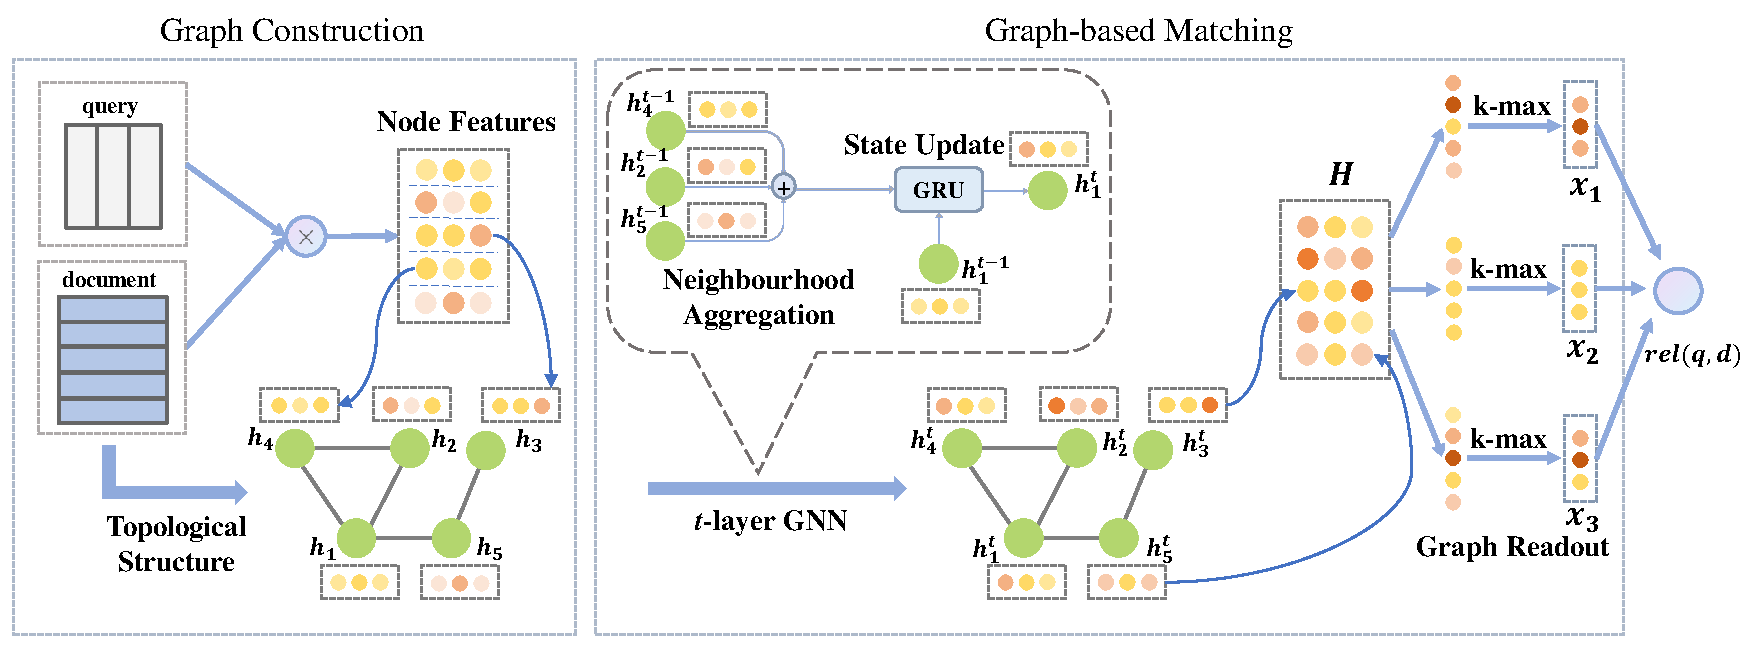
\includegraphics[width=\textwidth]{./pics/grmm.pdf}
	\caption{The workflow of the GRMM model. The document is first transformed into the graph-of-word form, where the node feature is the similarity between the word and each query term. Then, graph neural networks are applied to propagate these matching signals on the document graph. Finally, to estimate a relevance score, top-$k$ signals of each query term are chosen to filter out irrelevant noisy information, and their features are fed into a dense neural layer. }
	\label{fig:2} 
\end{figure*}

Nevertheless, the majority of existing neural matching models only take the linear text sequence, inevitably limiting the model capability. To this end, we propose to break the linear text format and represent the document in a flexible graph structure, where comprehensive interactions can be explicitly modeled. 



\subsection{Graph Neural Networks}
Graph is a kind of data structure which cooperates with a set of objects (nodes) and their relationships (edges). Recently, researches of analysing graphs with machine learning have attracted much attention because of its great representative power in many fields. 

Graph neural networks (GNNs) are deep learning based methods that operate in the graph domain. The concept of GNNs is previously proposed by  \cite{scarselli2008graph}. Generally, nodes in GNNs update own hidden states by aggregating neighbourhood information and mixing things up into a new context-aware state. There are also many variants of GNNs with various kinds of aggregators and updaters, such as \cite{li2016gated,kipf2017semi,hamilton2017inductive,velivckovic2018graph}. 

Due to the convincing performance and high interpretability, GNNs have become a widely applied structural analysis tool. Recently, there are many applications covering from recommendation \cite{wu2019session,li2019fi} to NLP area, including text classification \cite{yao2019graph,zhang2020every}, question answering \cite{de2019question}, and spam review detection \cite{li2019spam}.

In this work, we employ GNNs in the relevance matching task to extract implicit matching patterns from the query-document interaction signals, which is intrinsically difficult to be revealed by existing methods. 



\section{CLIP Embedding Space Analysis}
In this section, we present a detailed analysis of the CLIP embedding space. CLIP offers a pre-trained joint embedding space, enabling zero-shot vision-language tasks. However, there is still a \textit{modality gap} present in the CLIP embedding space \cite{MindGap}. This gap refers to a geometric property where image and text embeddings occupy distinct regions within the embedding space. We further analyze and demonstrate that the modality gap arises from an inherent ambiguity in matching visual and linguistic embeddings. Empirically, we show that integrating subregion image information with global information can reduce the gap between linguistic and visual representations. Additionally, we explore the disparity between CLIP's text and image representations, conducting an empirical study that reveals the difference follows a Gaussian distribution. These findings inspire our subsequent method design.
  
%\subsection{Preliminary of Modality Gap}
% -----------------------------------------------------------------------
% CLIP通过在大规模数据上的contrastive language-Image pretraining获得了joint embedding space,但这个joint embedding space上仍然有modality gap. modality gap指在clip embedding space中,text embedding和image embedding中间仍然存在gap。这种gap存在的原因是CLIP的预测始终会存在mismatch image text pair,这些mismatched pair的存在使得contrastive loss有保留这样的modality gap(有mismatch data的前提下,保留一定的modality gap使得contrastive loss达到global minimum)
% -----------------------------------------------------------------------
%CLIP obtain a joint embedding space by contrastive language-Image pretraining on a large dataset of images and their corresponding text descriptions. However 

\begin{figure}[t!]
  \centering
  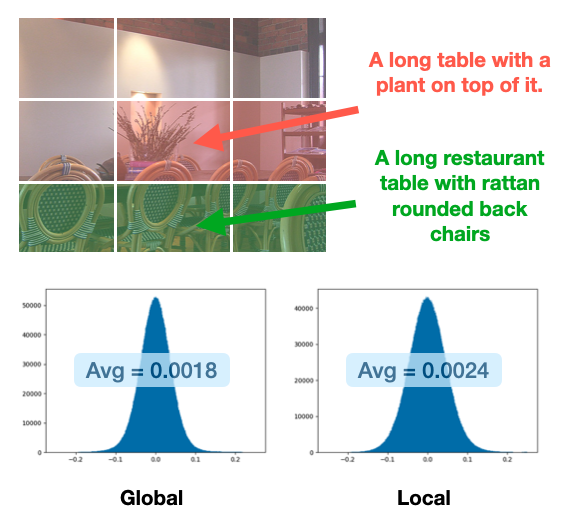
\includegraphics[width=0.35\textwidth]{AnonymousSubmission/LaTeX/asserts/ana_fig.png}
   \caption{The upper half of this figure is an example of the misalignment in paired image and text description. The lower half of this figure is the distribution of modality gap between text representation and global / local image representation respectively.}
    \label{figure:ex}
\end{figure}


\begin{table}[t]
\small
\centering
\tabcolsep=2pt
\begin{tabular}{c|ccc}
\toprule
\toprule
\multirow{2}{*}{} & \multicolumn{3}{l}{Pair Cosine Similarity} \\
                         & Mean        & Max        & Min        \\ \hline
 Global representation           & 0.330       & 0.446      & 0.228      \\ \hline

Mix representation             & 0.352       & 0.422      & 0.242      \\ \toprule
\end{tabular}
\caption{In this table, we show the mean, max and min value of similarity between text feature and global/mix feature. We find that after adding subregion information, the mean, max and min value all increase. This observation shows that introducing subregion image information benefit the alleviation of modality gap.}
\label{table:subregion}
\end{table}

\subsection{Modality Gap of CLIP Representations}
% \label{analysis:subregion}
% -----------------------------------------------------------------------
% modality gap的成因是mismatch pair。我们认为模型预测mismatch pair始终存在难以去除的原因是image和text两种模态表达的信息原本就是不对等的。具体地:1. 在annotation中认为是pair的image和text,text往往也并不描述image中的所有信息;2. text对图片描述了的部分,也难以避免歧义的发生;3. 并且对于同一个图片,也往往有多种进行文字描述的方法都是正确的,这些描述可能侧重图片的不同区域。这样的misalignment是固有的,因此是难以避免的。
% -----------------------------------------------------------------------

As demonstrated in \cite{MindGap}, the modality gap phenomenon is primarily caused by the presence of mismatched text-image data during pre-training, further exacerbated by the contrastive learning objective employed in CLIP. However, we observe that even correctly paired image-text may exhibit different semantic contents due to several reasons, including 1) incomplete image description by text; 2) ambiguity in text interpretation; 3) diverse valid descriptions with varying focus on image subregions. An example is illustrated in Figure~\ref{figure:ex}.
% Such modality misalignment is inherent, thus is hard to avoid. 
% -----------------------------------------------------------------------
% 基于这样的(mismatch image-text pair)的性质,我们可以利用subregion减弱modality gap带来的问题。我们假设对于某个具体地text description,一些subregion可能相比于global image有更小的gap。为了验证这个假设,我们进行了一些统计。我们计算global-text similarity和subregion-text similarity,取高的一个认为是匹配上了,我们发现有33%的subregion成功匹配上了。这样的结果验证了一些情况下subregion能有助于缩小modality gap
% -----------------------------------------------------------------------
%Based on the of characteristics, 
% we are able to alleviate the problems caused by modality gap by integrating CLIP visual feature with image subregion information. Given that the text description does not provide comprehensive representation of image and may focus on subregions of image, 
Consequently, we observe that certain subregions of an image typically exhibit a smaller modality gap with a specific text description, as illustrated in Figure~\ref{figure:ex}. To validate this characteristic, we conduct a statistical analysis on the MSCOCO validation set. Specifically, we calculate the cosine similarity between the visual and text features, where the visual features are obtained from the global CLS token or the last layer of the ViT encoder representing the subregions. The results indicate that in $\mathbf{33\%}$ of cases, one of the subregion features has a higher similarity than the global one.

%and embedded caption, visual patch feature and embedded caption feature. The visual patch features are from last layer of CLIP ViT encoder.
% the global-image-to-text similarity and subregion-to-text similarity. 
%A text description is said to be matched with the subregion if the similarity score of visual patch feature is higher, and vice versa. 

%We find that $\mathbf{33\%}$ of subregion representation successfully match with the text description. The results demonstrate the image subregion information may bring benefits to alleviate the modality gap. However, there still are $67\%$ cases the global representation achieve higher similarity score. 
%Consider that, we combine the global image representation and the local image representation by adding them together, and defined it as mix representation. We eval the similarity score between text representation and global/mix representation and show the results of mean, max and min score in Table~\ref{table:subregion}. We find that integrating subregion information leads to increase in mean score. This observation shows that introduce subregion image information benefit the alleviation of modality gap.

Motivated by the above observation, we propose integrating the global and subregion representations by adding them together. We evaluate the similarity scores between text features and their corresponding subregion-augmented image representations. As illustrated in Table~\ref{table:subregion}, our augmented image embeddings achieve higher similarity scores when compared with corresponding text embeddings without any fine-tuning, effectively reducing the modality gap.
% Specifically, we add the subregion representation to the global image representation. 
%The details will be presented in the \textit{Sub-region Feature Aggregation} section.
%As shown in our experiments, our sub-region augmented image embeddings achieve higher cosine similarity scores when compared with corresponding text embeddings without any fine-tuning.
% Below we will introduce our subregion-augmented embedding representation and a noise injection strategy to learn the mapping from image to text modality without paired data. 

\subsection{Distribution of Modality Gap}
% \label{analysis:Distribution_of_Modality_Gap}
We further investigate the distribution of the modality gap through an empirical study on the MSCOCO validation set. Specifically, for each image with its caption, we compute the difference between the image and text embeddings. We calculate these differences separately for the global image feature and the subregion feature. Given these differences, we pool all the feature dimensions together and compute a histogram and mean of the dimension-wise differences between the two modalities. As depicted in the lower half of Figure~\ref{figure:ex}, we observe that the mean of the gap distribution is close to zero, and the overall distribution resembles a Gaussian distribution for both global and subregion representations. Based on this observation, we adopt a unimodal learning strategy that involves Gaussian noise injection with the text features. This strategy allows us to mimic the image features in the cross-modal inference stage. For a more formal description of our analysis, please refer to the supplementary material.


%We have text modality representation $T^i \in \mathbb{R}^D$ and vision modality representation. To be noticed, for vision modality we have two set of representation: the global embedding representing the overall information and the patch embeddings representing the image subregions information. The global embedding is $I_c^i \in \mathbb{R}^D$, and the patch embedding is $I_p^i \in \mathbb{R}^{N \times D}$. Both global embedding and local embedding are obtained by CLIP. $D$ is the dimension of CLIP embedding and $N$ is the sequence length of CLIP. $i \in \{1, 2, ... , num\_samples\}$

%For paired images and text descriptions, we evaluate the gap between text representation and both global and patch image representation. For each image-text pair, we compute $G^c_i = T^i - I_c^i$ and $G^p_i = repeat(T^i, N) - I_p^i$. $G^c_i \in \mathbb{R}^{D}$, $G^p_i \in \mathbb{R}^{N \times D}$.

%We can check the overall distribution over all $D$ dimension. In this case, we treat data in all dimension equally. We compute the mean over all image-text pairs and draw the histgram of the data distribution. Thus we compute mean of the gap distribution for global vision and language representation as $Avg_{(i, d)} (I_c^i[d])$, and the gap for local vision and language representation as $Avg_{(i, s, d)} (I_p^i[s][d])$. $s \in [N], d \in [D]$ The results are shown in the lower half of  Figure~\ref{figure:ex}.

%The mean of the gap distribution between language and both global and local representation are close to zero. In Figure we sample $5e6$ example data and show the distribution, which is close to a Gaussian distribution. Based on this characteristic, we assume the modality gap distribution conforms to the Gaussian distribution. We are able to make the text representation closer to image representation by adding an appropriate Gaussian distribution.

\begin{figure*}[t!]
  \centering
  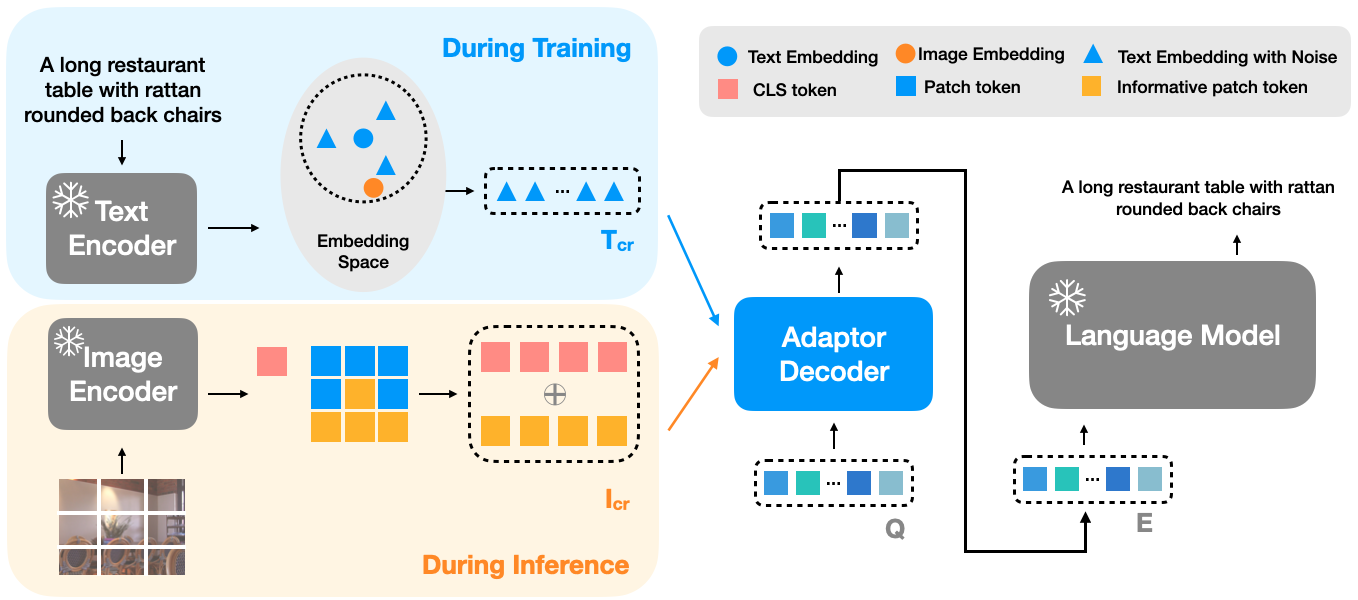
\includegraphics[width=0.7\textwidth]{AnonymousSubmission/LaTeX/asserts/new_pipeline.png}
   \caption{\textbf{An overview of MacCap pipeline.} MacCap learns to generate text based on region noise injected CLIP text feature in text reconstruction training. During inference, MacCap can generate caption without paired data in training. The CLIP and language model are kept frozen in both stages. }
    \label{figure:pipeline}
\end{figure*}

\section{Methods}

\subsection{Problem Formulation}
In crop yield prediction, we denote each county's climatic features by $\mathbf{x}_{c,t}$ and ground-truth crop yield (for a particular crop) by $y_{c,t}\in \mathbb{R}$, where $c$, $t$ represent county and year respectively. Each $\mathbf{x}_{c,t}$ contains four types of features (detailed descriptions of these features can be found in the Experiments section): weather features $\mathbf{x}_{c,t}^w\in \mathbb{R}^{n_w\times 52}$, land surface features $\mathbf{x}_{c,t}^l\in \mathbb{R}^{n_l\times 52}$, soil quality features $\mathbf{x}_{c}^s\in \mathbb{R}^{n_s\times 6}$, and some extra features (e.g. crop production index) $\mathbf{x}_{c}^e\in \mathbb{R}^{n_e}$. Namely, $\mathbf{x}_{c,t}=(\mathbf{x}_{c,t}^w, \mathbf{x}_{c,t}^l, \mathbf{x}_{c}^s, \mathbf{x}_{c}^e)$. We denote the number of weather, land surface, soil quality, and extra variables as  $n_w, n_l, n_s, n_e$ respectively. Among these features, $\mathbf{x}_{c,t}^w, \mathbf{x}_{c,t}^l$ change both spatially and temporally, while $\mathbf{x}_{c}^s, \mathbf{x}_{c}^e$ are county-specific and remain stable over time. The goal is to predict $y_{c,t}$ given $\mathbf{x}_{c,t}$. Recent work \cite{khaki2020cnn} also showed features from past years can help with the prediction, so we reformulate our task as predicting $y_{c,t}$ with $\{\mathbf{x}_{c,t},\mathbf{x}_{c,t-1},...,\mathbf{x}_{c,t-\Delta t}\}$. $\Delta t$ is the length of year dependency. If $\Delta t=0$, the model will not consider features from prior years. 

\subsection{Per-Year Embedding Extraction}
Regardless of whether the models use historical features or not, the first step is always to extract an embedding for each year from $\mathbf{x}_{c,t}$. Then a prediction can be made based on the embedding from the current year or the embeddings from the last few years.

The four types of features $\mathbf{x}_{c,t}^w, \mathbf{x}_{c,t}^l, \mathbf{x}_{c}^s, \mathbf{x}_{c}^e$ have different structures. Using a uniform neural network to extract the embedding may not effectively exploit the structure in the raw data. For example, weekly features $\mathbf{x}_{c,t}^w, \mathbf{x}_{c,t}^l$ naturally incorporate a temporal order, but county-specific soil features $\mathbf{x}_{c}^s$ do not change temporally and are measured at different depths underground. Therefore, we use separate neural networks to process the differently structured-parts from $\mathbf{x}_{c,t}$:
\begin{equation}
\label{eq:cnn}
\begin{aligned}
&\mathbf{h}_{c,t}^{wl}=f_{wl}(\mathbf{x}_{c,t}^w, \mathbf{x}_{c,t}^l) \\
&\mathbf{h}_{c}^s=f_s(\mathbf{x}_{c}^s) \\
&\mathbf{h}_{c,t}=(\mathbf{h}_{c,t}^{wl}, \mathbf{h}_c^s, \mathbf{x}_{c}^e)
\end{aligned}
\end{equation}
$f_{wl}(\cdot)$ handles the features that vary over time. Since land surface features like soil moisture from $\mathbf{x}_{c,t}^l$ are weekly data closely related to weather, we concatenate $\mathbf{x}_{c,t}^l$ and $\mathbf{x}_{c,t}^w$ before further passing to $f_{wl}$. Given the temporal order, an RNN or a CNN can be used for $f_{wl}$ to facilitate information aggregation along the time axis. On the other hand, $f_s(\cdot)$ aggregates information along soil depths. We use CNN as the architecture for $f_s$. $\mathbf{x}_{c}^e$ only contains six scalar values, so we directly pass it to the output embedding. The final embedding $\mathbf{h}_{c,t}$ is the concatenation of $\mathbf{h}_{c,t}^{wl}, \mathbf{h}_c^s, \mathbf{x}_{c}^e$.


\begin{figure*}[t]
\centering
\begin{minipage}[c]{7cm}
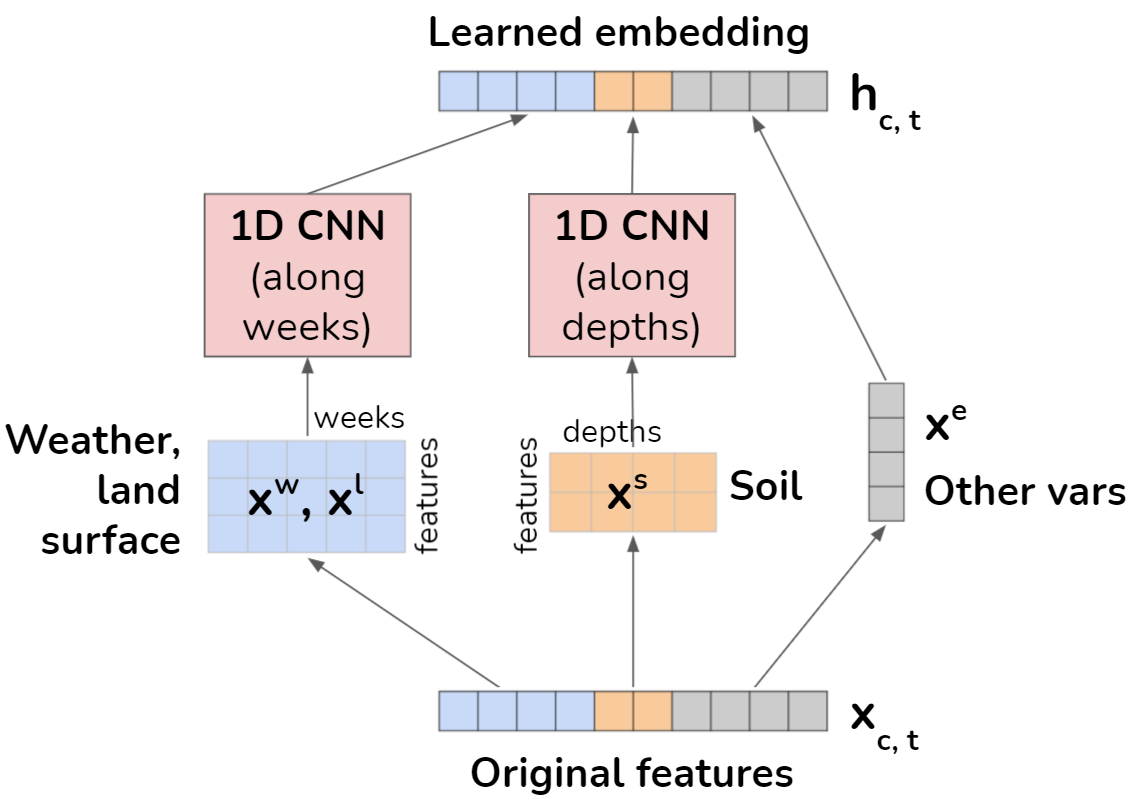
\includegraphics[width=6.9cm]{figs/cnn.png}
\label{fig:cnn}
\end{minipage}
\begin{minipage}[c]{10cm}
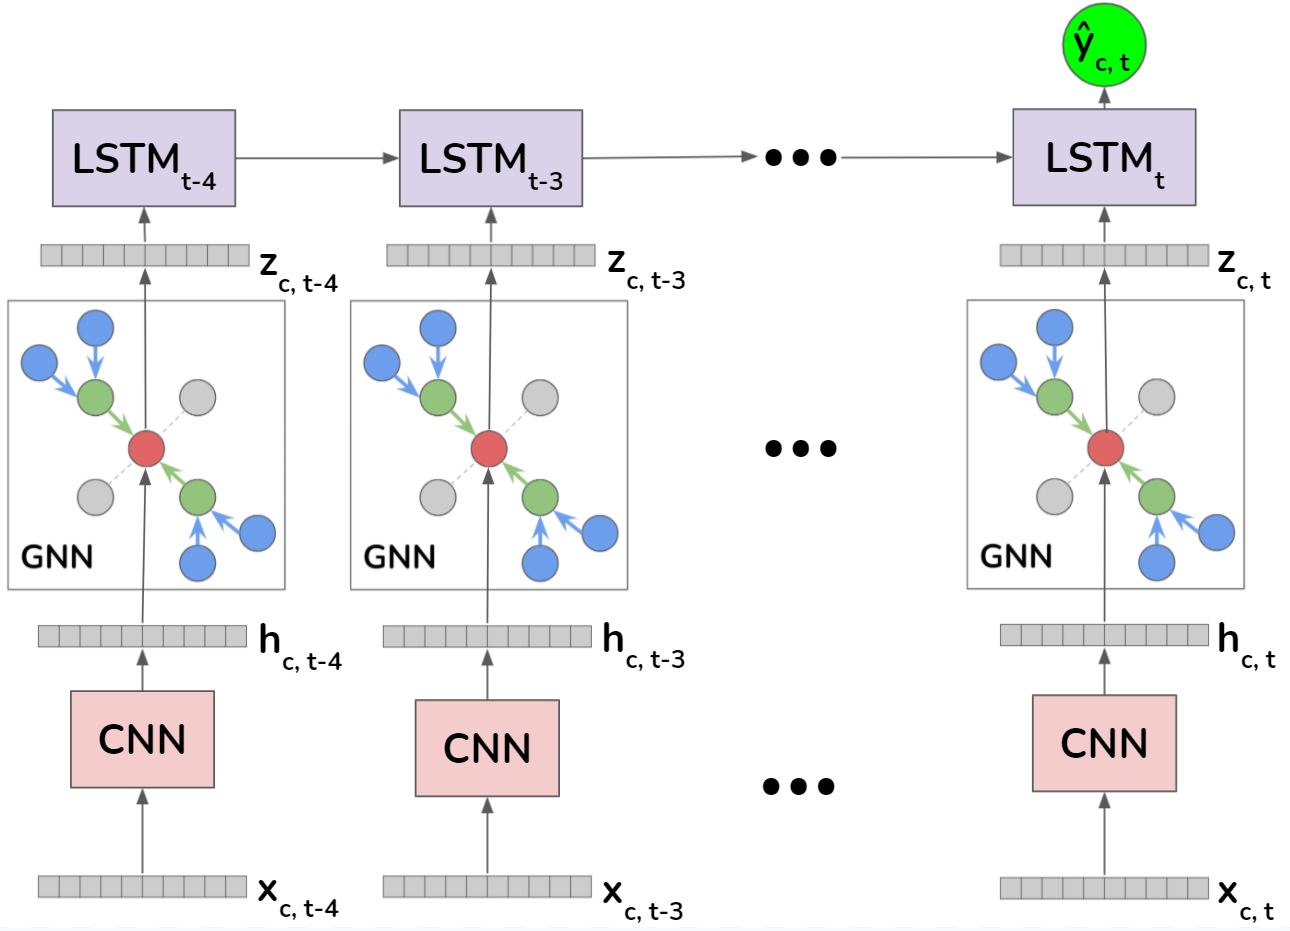
\includegraphics[width=9.9cm]{figs/gnn-rnn.png}
\label{fig:gnn-rnn}
\end{minipage}
\caption{\textbf{Left}: The CNN model used for per-year embedding extraction. \textbf{Right}: Our overall GNN-RNN framework. For each county $c$ and year $t'$, the CNN extracts an embedding $\mathbf{h}_{c, t'}$. Then we apply a GNN to refine each year's embedding by aggregating information from neighboring counties, producing a new embedding $\mathbf{z}_{c, t'}$. Finally, an LSTM processes the embeddings from each year and outputs the yield prediction $\widehat{y}_{c, t}$.}
\end{figure*}


\subsection{Temporal Dependency}
Though new crops are planted every year and yields primarily depend on climatic factors within one year, it has been observed that the trend and variations captured by recent history can be very informative for prediction \cite{khaki2020cnn}. For example, crop yields have tended to increase over the past few decades due to improvements in technology and genetics \cite{ortiz2018another}. While data on the underlying technological improvement is unavailable \cite{khaki2020cnn}, we can observe recent trends in crop yield. Our per-year embedding extraction makes it easy to incorporate  historical knowledge. All we need is an RNN that reads the per-year embeddings from the current year and several prior years. The output from the last time step would be our prediction for the crop yield of the current year: 
\begin{equation}
\label{eq:rnn}
\begin{aligned}
\widehat{y}_{c,t}=r(\mathbf{h}_{c,t-\Delta t}, ..., \mathbf{h}_{c,t-1}, \mathbf{h}_{c,t})
\end{aligned}
\end{equation}
where $r(\cdot)$ is an RNN, and $\mathbf{h}_{c,t'}$ is the embedding from year $t'$ for county $c$. The model described so far follows the CNN-RNN framework, which has previously been shown to outperform single-year NN models \cite{khaki2020cnn}.


\subsection{Incorporating Geographical Knowledge}
Eq.~\ref{eq:rnn} shows how one can extend the use of embeddings from Eq.~\ref{eq:cnn} temporally. Then a natural question is, Can we take advantage of the embeddings geospatially as well? Intuitively, if a county has good yields, nearby counties tend to have good yields as well. The weather and soil conditions should also transition smoothly across the continent. The additional features from neighboring counties could boost the prediction if used properly. A recent success in COVID-19 forecasting \cite{kapoor2020examining} with similar insights could further support incorporating geographical knowledge, where the graph-based representation learning greatly improves case prediction. 

\subsubsection{Graph Neural Network}
Graph Neural Network (GNN) \cite{zhou2020graph} is a novel type of neural network proposed to unravel the complicated dependencies inherent in graph-structured data sources.
%GNN allows more flexibility and a wider representation space to embed the node and edge information from the graph for inference.
Given its strong power in representation learning, GNN has demonstrated prominent applications in chemistry \cite{gilmer2017neural}, traffic \cite{cui2019traffic}, biology \cite{fout2017protein}, and computer vision \cite{satorras2018few} with sophisticated model architectures \cite{kipf2016semi,hamilton2017inductive,velivckovic2017graph}. Formally, a graph is denoted by $G=(V,E)$ where $V$ is the set of nodes and $E$ is the set of edges between nodes. In our crop yield prediction task, each node is a county. $E$ is represented as a symmetric adjacency matrix $A\in \{0,1\}^{N\times N}$ where $A_{i,j}=1$ if two counties $v_i, v_j\in V$ border and $A_{i,j}=0$ otherwise. $N$ is the total number of counties. Each node is associated with $\mathbf{x}_{c,t}$ for every year. 

\subsubsection{GraphSAGE} 
A popular GNN model, GraphSAGE, \cite{hamilton2017inductive} is a general framework that leverages node feature information and learns node embeddings through aggregation from a node's local neighborhood. Unlike many other methods based on matrix factorization and normalization \cite{jia2020residual}, GraphSAGE simply aggregates the features from a local neighborhood, and is thus less computationally expensive. The features can be aggregated from a different number of hops or search depth. Therefore the model often generalizes better. GraphSAGE is suitable for crop yield prediction because most counties only border a few others and the adjacency matrix is sparse. It also provides flexible aggregation methods.

Formally, for the $l$-th layer of GraphSAGE, 
\begin{equation}
\label{eq:gnn}
\begin{aligned}
&\mathbf{a}_{c,t}^{(l)} = g_l(\{\mathbf{z}_{c',t}^{(l-1)},\forall c'\in\mathcal N(c)\})\\
&\mathbf{z}_{c,t}^{(l)} = \sigma(\mathbf{W}^{(l)}\cdot (\mathbf{z}_{c,t}^{(l-1)}, \mathbf{a}_{c,t}^{(l)}))
\end{aligned}
\end{equation}
where $\mathbf{z}_{c,t}^{(0)}=h_{c,t}$ from Eq.~\ref{eq:cnn}, and $l\in\{0,1,...,L\}$. $\mathcal N(c)=\{c', \forall A_{c,c'}=1\}$ is the set of neighboring counties for $c$. The aggregation function for the $l$-th layer is denoted $g_l(\cdot)$, which could be mean, pooling, or graph convolution (GCN) function. In practice, we found mean or pooling are effective and computationally efficient. $\mathbf{a}_{c,t}^{(l)}$ is the aggregated embedding from the bordering counties. We concatenate $\mathbf{a}_{c,t}^{(l)}$ with the last layer's embedding $\mathbf{z}_{c,t}^{(l-1)}$ before the transformation using $\mathbf{W}^{(l)}$. $\sigma(\cdot)$ is a non-linear function.

\subsubsection{GNN-RNN}
The output embedding from GNN's last layer $\mathbf{z}_{c,t}^{(L)}$ thus extracts the information (e.g., weather, soil) from the whole local neighborhood for year $t$. To integrate the historical knowledge, we can do the same as in Eq.~\ref{eq:rnn}, by taking the GNN output embeddings from prior years:
\begin{equation}
\label{eq:gnn-rnn}
\begin{aligned}
\widehat{y}_{c,t}=r(\mathbf{z}_{c,t-\Delta t}^{(L)}, ..., \mathbf{z}_{c,t-1}^{(L)}, \mathbf{z}_{c,t}^{(L)})
\end{aligned}
\end{equation}
where $\mathbf{z}_{c,t'}^{(L)}$ is the GNN embedding from year $t'$.

\subsubsection{Loss Function}
We use log-cosh function as our objective:
\begin{equation}
\begin{aligned}
L(\widehat{y}_{c,t}, y_{c,t})=\log(\text{cosh}(\widehat{y}_{c,t}-y_{c,t}))
\end{aligned}
\end{equation}
Log-cosh works similarly to mean square error, but is not as strongly affected by the occasional wildly incorrect prediction. It is also twice differentiable everywhere. Mini-batch training is adopted during optimization. Batch loss is the average log-cosh loss of all samples in a batch. 


\section{Experiments}
\label{sec:experiment}

\begin{table}[t]
\centering
\small
\resizebox{0.99\linewidth}{!}{
\begin{tabular}{lcccc}
\multirow{2}{1.5cm}{\textbf{Methods}} & \multicolumn{2}{c}{\textbf{Far-OOD}} & \multicolumn{2}{c}{\textbf{Near-OOD}}\\
\cmidrule{2-5}
& \textbf{FPR95}  & \textbf{AUROC} & \textbf{FPR95}  & \textbf{AUROC}\\
& $\downarrow$ & $\uparrow$ & $\downarrow$ & $\uparrow$ \\
\toprule
\emph{Using model outputs}\\
MSP~\cite{hendrycks2016baseline} & 52.11 & 91.79 & 64.66 & 85.28 \\
ODIN~\cite{liang2018enhancing}  & 26.47 & 94.48 & 52.32 & 88.90\\
GODIN~\cite{hsu2020generalized}  & 17.42  & 95.84 & 60.69 & 82.37 \\
Energy score~\cite{liu2020energy}  & 28.40 & 94.22 & 50.64 & 88.66 \\
ReAct~\cite{sun2021react} & 33.12 & 94.32 & 53.51 & 88.96\\
GradNorm~\cite{huang2021importance} & 24.79 & 92.58 & 65.44 & 79.31\\
LogitNorm~\cite{wei2022mitigating}  & 19.61 & 95.51 & 55.08 & 88.03\\
DICE~\cite{sun2022dice}  & 20.83 & 95.24 & 58.60 & 87.11 \\
\midrule
\emph{Using feature representations}\\
Mahalanobis~\cite{lee2018simple} & 44.55 & 82.56 & 87.71 & 78.93 \\
KNN~\cite{sun2022knn}  & 18.50 & 96.36 & 58.34 & 87.90 \\
\midrule 
 \name (ours) & \textbf{14.99} & \textbf{97.15}  & \textbf{50.10} &  \textbf{89.80}\\
 & $\pm{0.87}$ & $\pm{0.27}$ & $\pm{1.09}$ & $\pm{0.65}$\\
\bottomrule
\end{tabular}}
\caption{\small Performance comparison on near-OOD and far-OOD detection task. Architecture used is DenseNet-101 and ID data is CIFAR-10. We report the mean and variance across 3 training runs.}
\label{tab:hard_ood}
\end{table}
\begin{table}[t]
\small
\centering
\resizebox{0.99\linewidth}{!}{
\begin{tabular}{lccc}
\textbf{Method} & \textbf{FPR95}  & \textbf{AUROC} & \textbf{ID Acc.}\\
& $\downarrow$ & $\uparrow$ & $\uparrow$ \\
\toprule
\emph{Methods using model outputs}\\
MSP~\cite{hendrycks2016baseline} & 77.59 & 76.47 &  75.14\\
ODIN~\cite{liang2018enhancing} & 56.39 & 86.02 & 75.14\\
GODIN~\cite{hsu2020generalized} & 44.08 &  89.05 & 74.37\\
Energy score~\cite{liu2020energy} & 57.07 &  84.83 &  75.14\\
ReAct~\cite{sun2021react} & 75.06 & 79.51 & 66.56\\
GradNorm~\cite{huang2021importance} & 63.05 & 79.80 & 75.14\\
LogitNorm~\cite{wei2022mitigating} & 61.10 & 84.72 & 75.42\\
DICE~\cite{sun2022dice} & 49.72 & 87.23 & 68.65 \\
\midrule 
\emph{Methods using feature representations}\\
Mahalanobis~\cite{lee2018simple} & 56.93 & 80.27 &  75.14\\
KNN~\cite{sun2022knn} & 47.21 & 85.27 & 75.14\\
\midrule 
 \name (ours) & \textbf{31.25} & \textbf{90.76} & \textbf{75.59}\\
& $\pm{1.25}$ & $\pm{0.36}$ & $\pm{0.08}$\\
\bottomrule
\end{tabular}}
\caption{\small Performance comparison on CIFAR-100 dataset. We use DenseNet-101 for all baselines. Best  results are in \textbf{bold}. We report the mean and variance across 3 different training runs.}
\label{tab:cifar-100}
\end{table}
In this section, we extensively evaluate the effectiveness of our proposed method. 
The goal of our experimental sections is to mainly answer the following questions: (1) Can \name alleviate the curse of dimensionality? (2) How does \name compare against the state-of-the-art OOD detection methods?  Due to space constraints, extensive experimental details are in Appendix C. Our code is open-sourced for the research community.


\subsection{Evaluation on Common Benchmarks}
\label{subsec:common_benchmark}

\noindent \textbf{Datasets.} In this section, we make use of commonly studied CIFAR-10 (10 classes) and CIFAR-100 (100 classes)~\cite{krizhevsky2009learning} datasets as ID. Both datasets consist of images of size $32 \times 32$. We use the standard split with $50,000$ images for training and $10,000$ images for testing. We evaluate the methods on common OOD datasets: \texttt{Textures}~\cite{cimpoi2014describing}, \texttt{SVHN}~\cite{svhn}, \texttt{LSUN-Crop}~\cite{yu2015lsun}, \texttt{LSUN-Resize}~\cite{yu2015lsun}, \texttt{iSUN}~\cite{xu2015turkergaze}, and \texttt{Places365}~\cite{zhou2017places}. Images in all these test datasets are of size $32 \times 32$. 


\paragraph{Evaluation metrics.} We compare the performance of various methods using the following metrics: 
(1) {FPR95} measures the false positive rate (FPR) of OOD samples when $95\%$ of ID samples are correctly classified;
(2) {AUROC} is the area under the Receiver Operating Characteristic curve; 
and (3) {ID Acc.} measures the ID classification accuracy.

\vspace{0.2cm}
\noindent \textbf{Comparison with competitive methods.} In Table~\ref{tab:cifar-100}, we provide a comprehensive comparison with competitive OOD detection baselines on  CIFAR-100. {We provide a detailed description of baseline approaches in Appendix C.3.} We observe that our proposed method \name significantly outperforms the latest rivals. For a fair comparison, we divide the baselines into two categories: methods using model outputs and methods using feature representations.
From Table~\ref{tab:cifar-100}, we highlight two salient observations: (1) Considering methods based on feature representations, \name outperforms KNN (non-parametric) and Mahalanobis (parametric) by \textbf{15.96\%} and \textbf{25.68\%} respectively in terms on FPR95. The results validate that learning feature subspace effectively alleviates the ``curse-of-dimensionality" problem that is troubling the existing KNN approach. (2) Further, \name also performs better than output-based methods such as ReAct~\cite{sun2021react}. Specifically, with CIFAR-100 as ID, \name provides a $\mathbf{43.81}\%$ improvement in FPR95 as compared to ReAct~\cite{sun2021react}. Notably, \name provides a \textbf{18.47\%} improvement compared to~\cite{sun2022dice}, a post-hoc sparsification method. While DICE can severely affect the ID test accuracy (68.65\%), \name exhibits stronger classification performance (75.59\%) by baking in the inductive bias of subspaces through training. An extensive discussion is provided in Section~\ref{sec:discussion}. 



\paragraph{Evaluation on near-OOD data.} In Table~\ref{tab:hard_ood}, we compare the performance in detecting near-OOD data, which refers to samples near the ID data. Near-OOD is particularly challenging to detect, and can often be misclassified as ID. We report the performance on CIFAR-10 (ID) vs. CIFAR-100 (OOD), which is the most commonly used dataset pair for this task. We observe that \name consistently outperforms existing algorithms for near-OOD detection tasks, further demonstrating its strengths. Compared to KNN, \name reduces the FPR95 by 8.24\%. For completeness, we also provide far-OOD evaluation results on CIFAR-10, where \name achieves an average FPR95 of 14.99\%. Full result on each test dataset for CIFAR-10 is available in Appendix D.4.



\begin{table}[t]
\small
\centering
\resizebox{0.95\linewidth}{!}{
\begin{tabular}{lccc}
\textbf{Method} & \textbf{Dataset (ID)} & \textbf{FPR95}  & \textbf{AUROC} \\
& & $\downarrow$ & $\uparrow$  \\
\toprule
Mahalanobis~\cite{lee2018simple} & CIFAR-10 & 44.55 & 82.56  \\

\name (w. Mahalanobis) & CIFAR-10 &  \textbf{34.68} &  \textbf{87.87} \\
\midrule
Mahalanobis~\cite{lee2018simple} & CIFAR-100 & 56.93 & 80.27  \\

\name (w. Mahalanobis) & CIFAR-100 &  \textbf{55.05} &  \textbf{80.77} \\
\bottomrule
\end{tabular}}
\caption{\small \name is also compatible with parametric approaches such as Mahalanobis distance~\cite{lee2018simple}. The model is DenseNet. All values are averaged over six OOD test datasets.}
\label{tab:compatibility}
\end{table}


\paragraph{Compatibility with other distance-based approaches.} 

Beyond KNN~\cite{sun2022knn}, the Mahalanobis distances~\cite{lee2018simple} is also one of the most popular distance-based approaches to detect OOD. 
However, all prior solutions measure the distance with a full feature space which can also suffer from the curse of dimensionality. 
In this section, we show that subspace learning can also benefit parametric approaches like Mahalanobis distance~\cite{lee2018simple}. In Table~\ref{tab:compatibility}, we compare the OOD detection performance of using Mahalanobis distance on the vanilla model and the model trained with \name. 
We see that coupling subspace learning (in training) with Mahalanobis distance (in testing) reduces FPR95 by {9.87\%} and {1.88\%} on CIFAR-10 and CIFAR-100 datasets respectively.

\begin{table}[t]
\small
\centering
\resizebox{0.55\linewidth}{!}{
\begin{tabular}{lcc}
\toprule
\multirow{2}{2cm}{\textbf{Training Method}} &  CIFAR-10 & CIFAR-100 \\ 
& \multicolumn{2}{c}{(Train time in hours)} \\
\midrule
Standard & $2.10$ & $2.25$\\ 
 \name & $1.75$ & $1.89$ \\
\bottomrule
\end{tabular}}
\caption{\small \textbf{Computational cost for training}. trained using ResNet-101. 
Model used is DenseNet-101. For the comparison, we used the software configuration as reported in Appendix C.2.}
\label{tab:train_time}
\end{table}
% 
\paragraph{Computational complexity.}  In Table~\ref{tab:train_time}, we compare the training time of \name with the standard training method using cross-entropy loss. We observe that training using \name incurs no additional computation overhead but rather is slightly more efficient compared to standard training procedures. This is because we perform gradient descent only on a subset of weights corresponding to the selected feature subspace. Thus, our method overall leads to faster updates and convergence. {In Appendix D.1, we further show that
\name remains competitive and outperforms the KNN counterpart on other common architecture.}

\section{Conclusion}
In this paper, we introduced a new ad-hoc retrieval approach GRMM which explicitly incorporates document-level word relationships into the matching function. The flexible graph structure allows the model to find more comprehensive matching patterns and less noises. GRMM exceedingly advances the performance over various baselines, where it empirically witnesses an increment by a large margin on longer documents. Further studies exhibited the rationality and effectiveness of GRMM. There are also possible extensions, such as training with large click logs \cite{jiang2016learning} and query descriptions. Another interesting future work is to extend the current graph with lexical or knowledge graphs which might contain more useful information. 

\bibliography{aaai24}

\end{document}
